\documentclass[journal,twoside,10pt]{IEEEtran}

% Packages
\usepackage{cite}
\usepackage[T1]{fontenc}
\usepackage{url}
\usepackage{amsmath,amssymb,amsfonts}
\usepackage{algorithmic}
\usepackage{graphicx}
\usepackage{textcomp}
\usepackage{xcolor}
\usepackage{listings}
\usepackage{afterpage}

% Custom section formatting for IEEEtran
\makeatletter
% Use Roman numerals for sections
\renewcommand\thesection{\Roman{section}}
% Format sections with Roman numerals and add period
\renewcommand\section{\@startsection{section}{1}{\z@}%
                       {-3.5ex \@plus -1ex \@minus -.2ex}%
                       {2.3ex \@plus.2ex}%
                       {\normalfont\Large\bfseries\Roman{section}.\quad}}
% Keep subsections unnumbered with no dot
\renewcommand\thesubsection{}
% Redefine subsection to avoid using any numbering
\renewcommand\subsection{\@startsection{subsection}{2}{\z@}%
                       {-3.25ex\@plus -1ex \@minus -.2ex}%
                       {1.5ex \@plus .2ex}%
                       {\normalfont\large\bfseries}}
% Empty section format to prevent automatic numbering
\renewcommand\@seccntformat[1]{}
\makeatother

% Configure listings package with enhanced JSON styling
\lstdefinestyle{mystyle}{
    backgroundcolor=\color{gray!10},
    commentstyle=\color{green!50!black},
    keywordstyle=\color{blue},
    stringstyle=\color{purple},
    basicstyle=\ttfamily\small,
    breakatwhitespace=false,
    breaklines=true,
    captionpos=b,
    keepspaces=true,
    numbers=none,
    numbersep=5pt,
    showspaces=false,
    showstringspaces=false,
    showtabs=false,
    tabsize=2
}

% Custom JSON styling
\lstdefinelanguage{JSON}{
    morestring=[b]",
    stringstyle=\color{purple},
    showstringspaces=false,
    keywords={false,true,null},
    keywordstyle=\color{orange},
    morekeywords={[2]"task_id","task","plan","actions","step","controlLabel","controlText","function","args","file_path"},
    keywordstyle={[2]\color{blue}},
    sensitive=false,
    comment=[l]{//},
    commentstyle=\color{green!50!black},
    morecomment=[s]{/*}{*/},
    literate=
        {:}{{{\color{black}{:}}}}{1}
        {,}{{{\color{black}{,}}}}{1}
        {\{}{{{\color{black}{\{}}}}{1}
        {\}}{{{\color{black}{\}}}}}{1}
        {[}{{{\color{black}{[}}}}{1}
        {]}{{{\color{black}{]}}}}{1}
}

\lstset{style=mystyle}

\begin{document}

\title{A State-of-the-Art Survey on AI Systems for Multi-Task Productivity: From Large Language Models to Multi-Agent Systems}

\author{Your Name \\ Your Affiliation}

\maketitle

\begin{abstract}
The rapid evolution of large language models (LLMs) has catalyzed the development of systems capable of performing multiple productive tasks. Early breakthroughs in language modeling paved the way for models to autonomously select and utilize external tools. Subsequent research focused on transforming these models into Large Action Models (LAMs) tailored for action execution. More recently, integrating LAMs within multi-agent systems (MASs) has emerged as a promising strategy for tackling complex, real-world tasks. This survey synthesizes historical progress, contemporary research, and future directions in the field—from LLMs using tools to MASs that achieve collaborative, autonomous task execution.
\end{abstract}

\begin{IEEEkeywords}
LLMs, Toolformer, ToolLLM, Large Action Models, Multi-Agent Systems, Autonomous Agents, Collaborative AI
\end{IEEEkeywords}

\section{Introduction}
Large language models (LLMs) have redefined what is possible in artificial intelligence, demonstrating unprecedented capabilities in natural language understanding and generation. Despite their success, early LLMs were inherently limited to text-based outputs and struggled with tasks requiring real-world action. Recent work has demonstrated that LLMs can be extended to identify and call appropriate tools, effectively bridging the gap between language and action. This survey reviews the evolution from tool-using LLMs to specialized Large Action Models (LAMs), and ultimately to multi-agent systems that harness these capabilities for collaborative, productive task execution.

In the following sections, we outline:
\begin{itemize}
    \item \textbf{How we got here:} A brief history of LLMs' transformation through tool usage.
    \item \textbf{Where we are now:} The emergence of LAMs and their integration into multi-agent frameworks.
    \item \textbf{Where we could go next:} Challenges faced by current systems and potential directions for future research.
\end{itemize}

\section{Literature Review}

\subsection{From Language Models to Tool-Using Agents}

Advancements in artificial intelligence have accelerated in recent years, particularly with the introduction of the transformer architecture. This innovation enabled commercial LLM-supported products and significantly impacted society's understanding of AI. From a product engineering perspective, where user interface design is paramount and team value comes from well-crafted experiences, the chat interface has been widely embraced. This rapid adoption is no coincidence—our first interactions with LLMs occurred through interfaces that create the impression of conversing with another person, resulting in a natural experience that increased user adoption.

Initially, the value users derived from these interfaces was largely limited to text generation. As interactions became multimodal, the term "Generative AI" become popular to describe these systems. This term reflects both their architectural approach to generating outputs and their perceived intelligence and creativity—their ability to create new ideas, images, and sounds. This framing helps us understand phenomena like "hallucinations" and other characteristics of these AI systems.

In brief, contrary to science fiction's predictions, we have developed a form of artificial intelligence that excels more at creative tasks than logical ones. This observation sets the foundation for our literature review: while current AI shows immense potential, it still lacks the reliability needed for complex task execution.

In this research exercise, we identify a trend of evolution that expands around 3 years, i.e., \cite{schick2023toolformer, qin2023toolllm}. Researchers noticed the potential of the LLMs to be used for more than just text generation, as they display excellent ability to understand and produce structured output, there was a possibility of integrate with existing software artifacts already in place, such as APIs, SDKs, and any other programmable interface.

API's where one of the most natural places to start with.  Toolformer (Schick et al., 2023)~\cite{schick2023toolformer} represents a breakthrough in addressing LLM limitations through tool integration, enabling models to autonomously determine when external tools are needed, select appropriate ones, and incorporate their outputs into ongoing language generation. Its distinctive self-supervised learning methodology implements a streamlined three-step process that samples potential API calls using in-context learning, executes these calls to obtain results, and filters them based on perplexity reduction. This approach creates a more adaptive system capable of determining which tools benefit specific contexts without extensive human annotation.

Expanding this line of research, ToolLLM (Qin et al., 2023)~\cite{qin2023toolllm} introduces a comprehensive framework for training models to effectively utilize external tools through API calls. It contributes three key innovations: a systematic methodology for converting conventional dialogue datasets into tool-use examples through automated annotation; ToolBench, a diverse dataset spanning over 16,000 real-world scenarios across various domains; and a training approach enabling models to make effective API calls without human intervention. Performance evaluations demonstrate that tool-augmented models significantly outperform standard approaches, particularly in generating syntactically correct API calls, tool selection, and output integration.

These complementary innovations mark a crucial first step in improving the reliability of AI systems for performing specific tasks by establishing a new paradigm where language models can handle tasks beyond linguistics to perform useful, real-world operations. By maintaining sophisticated language understanding while gaining access to specialized functionality, tool-augmented systems offer a cost-effective approach to enhancing model capabilities without increasing model size, potentially transforming how AI assistants support human productivity across diverse domains.

\subsection{Large Action Models (LAMs)}

Tool-using LLMs introduced a paradigm shift in the way we perceive the functionality of AI systems, the main idea was: "Now we have a system that can interact with our world",  in the context of our modern digital productivity tools. Taking a step further in the evolution of  an LLM using tools, our research found the concept of "Large Action Models" which introduces a new action layer that positions AI systems at the same level of interaction as modern application layers. This advancement has produced systems capable of performing actions in dynamic environments. Although LAMs did not require significant architectural changes to LLMs, the name effectively captured the new direction of applied AI. We now proceed to describe this process.

\subsubsection{Developing and Training Large Action Models}

The goal is to transform a general-purpose LLM into a specialized action execution system. This transformation requires designing a dedicated pipeline. Wang et al.~\cite{wang2025lam} describe this process in detail. Understanding this pipeline is important not only for this paper but also because these methods can be applied broadly to similar objectives, enriching our understanding for future development. The process consists of several interconnected stages:

\paragraph{Data Collection and Preparation}
As most of AI related work, everything starts with gathering and curating task-specific data. This initial phase follows a two-phase approach:

\begin{itemize}
    \item \textbf{Task-Plan Data Collection}: This involves collecting user requests and corresponding step-by-step plans. Sources include application documentation, WikiHow articles, and historical search queries. Each entry typically contains a task description and a detailed plan outlining the steps required to accomplish it.
    
    \item \textbf{Task-Action Data Collection}: This phase converts task-plan data into executable task-action data. Each plan step is transformed into concrete, actionable instructions that can be directly executed in the target environment. This process includes instantiation (adding specific operational details), execution validation, and evaluation to ensure correctness.
\end{itemize}

For example, a typical entry might look like:

\begin{lstlisting}[language=JSON]
{
  "task_id": "powerpoint_task_001",
  "task": "Create a slide based on draft.docx",
  "plan": [
    "1. Open the draft.docx and read the content.",
    "2. Create a new PowerPoint file.",
    "3. For page 1, add ..."
  ],
  "actions": [
    {
      "step": "open the document",
      "function": "open",
      "args": {"file_path": "draft.docx"}
    }
  ]
}
\end{lstlisting}

\paragraph{Transforming an LLM into a LAM, a Four-Phase Approach}

\begin{figure}[htbp]
    \centering
    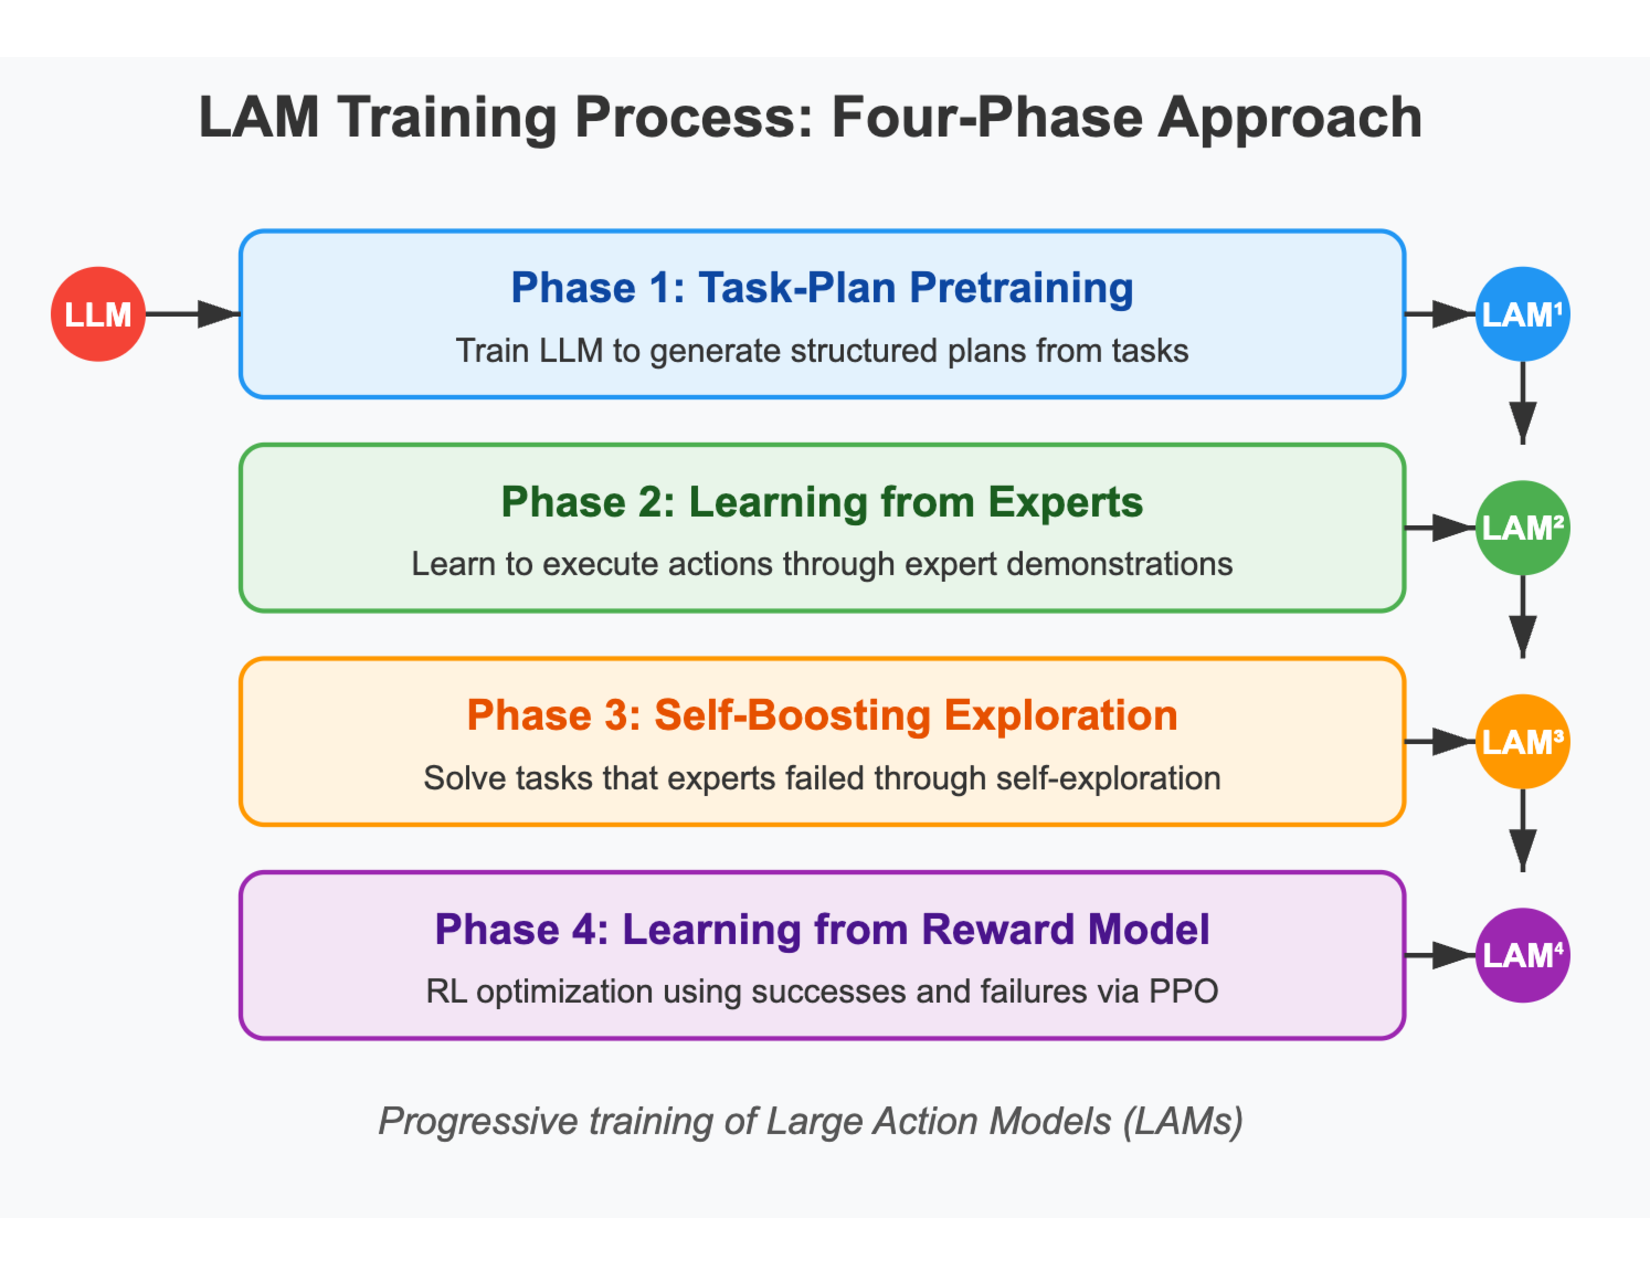
\includegraphics[width=0.5\textwidth]{traning_phases.pdf}
    \caption{Progressive four-phase training approach for transforming a general LLM into a specialized LAM.}
    \label{fig:lam-training}
\end{figure}

Wang et al.~\cite{wang2025lam} propose a systematic, four-phase training process that progressively builds capabilities from planning to action execution. As our LLM model progresses through these phases, it becomes a LAM:

\begin{enumerate}
    \item \textbf{Task-Plan Pretraining}: In this foundational phase, the model (LAM$^1$) learns to generate structured, step-by-step plans for completing tasks. Using supervised fine-tuning with task-plan pairs, the model develops the ability to break tasks into logical sequences. At this stage, the model can generate coherent plans but lacks execution capabilities.
    
    \item \textbf{Learning from Experts}: In the second phase, the model (LAM$^2$) learns to translate plans into concrete, executable actions through expert demonstrations. Training uses state-action pairs where each state includes the current UI environment and task context, and each action specifies which control to interact with and how. This phase grounds the model's reasoning in real application environments.
    
    \item \textbf{Self-Boosting Exploration}: In the third phase, the system learns to improve itself. LAM$^2$ attempts to solve tasks that were unsuccessful in previous stages. Using a ReAct mechanism, \cite{yao2022react}, it interacts with the environment and explores alternative strategies for these challenging tasks. When successful, it generates new solutions. These solutions are then combined with the original expert examples to create an enhanced training dataset for LAM$^3$.
    
    \item \textbf{Learning from a Reward Model}: The final phase introduces reinforcement learning, enabling the model to learn from both successes and failures. First, a reward model is trained on both successful and failed trajectories, assigning positive values to successful steps and negative values to failures. Then, LAM$^4$ is fine-tuned using Proximal Policy Optimization (PPO) on previously failed trajectories, guided by the reward model's feedback. This approach enhances the model's decision-making abilities in complex scenarios.
\end{enumerate}

Each step in the training process builds on the one before it. This creates AI systems that get better and better at four key things: Planning out steps to solve problems, learning from expert examples, figuring things out on their own, getting better through trial and error.

\paragraph{Integration with Agents}
Once the trained is complete, it is neccessary to close the breach between strategy and execution. In few words, we have a very capable model to engage in planning to resolve tasks, but it's necessary to add interaction with the environment where it will operate. We introduce the concept of Agents—though their meaning and specific definition are still evolving—which, in the context of this paper, represent a layer of interaction between LAMs and the environment. LAMs must be integrated into an agent framework to interact with real-world environments. To make LAMs work in the real world, they need four main parts working together:

\begin{enumerate}
    \item A way to see and understand what's happening in their environment, usually through special software interfaces (UI Automation APIs)
    \item A system that turns the model's decisions into actual actions in the environment
    \item A memory system that keeps track of what actions were taken and what plans were made, helping the system stay organized and consistent
    \item A feedback system that watches how the environment responds to actions, helping the system learn and adjust to changes
\end{enumerate}

Put simply, the LAM functions as the brain while the Agents serve as the body, complete with hands that can manipulate tools and execute plans.

\paragraph{Evaluation}
Evaluation is a critical component of any DL/ML system, serving as the feedback loop for system improvement. While Wang and colleagues~\cite{wang2025lam} established clear testing methodologies for comparing different versions and ensuring proper functionality across various situations, the current evaluation scope remains limited to a 435-task benchmark focused on Microsoft Word tasks. Nevertheless, their comprehensive development pipeline demonstrates LAMs' ability to translate user intentions into meaningful actions within specific operational contexts, representing a significant advancement over traditional text-generation models by enabling the execution of complex, multi-step tasks in real-world environments—though more extensive testing across diverse domains is still needed.

\subsubsection{Applications and Impact}
LAMs enable a wide range of applications previously challenging for traditional LLMs, including:

\begin{itemize}
    \item Autonomous interaction with software applications and operating systems
    \item Control of physical devices and robotic systems
    \item Complex task automation in specialized domains like healthcare or finance
    \item Multi-step problem-solving that requires environmental awareness
\end{itemize}

These capabilities mark a significant advancement toward artificial general intelligence (AGI), enabling AI systems to automate tasks that were previously only possible with human intervention.

LAMs thus represent a paradigm shift—from language generation to action execution—allowing AI systems to automate complex processes with minimal human intervention, substantially expanding their practical utility across numerous domains.

\subsection{Multi-Agent Systems}

\begin{figure}[htbp]
    \centering
    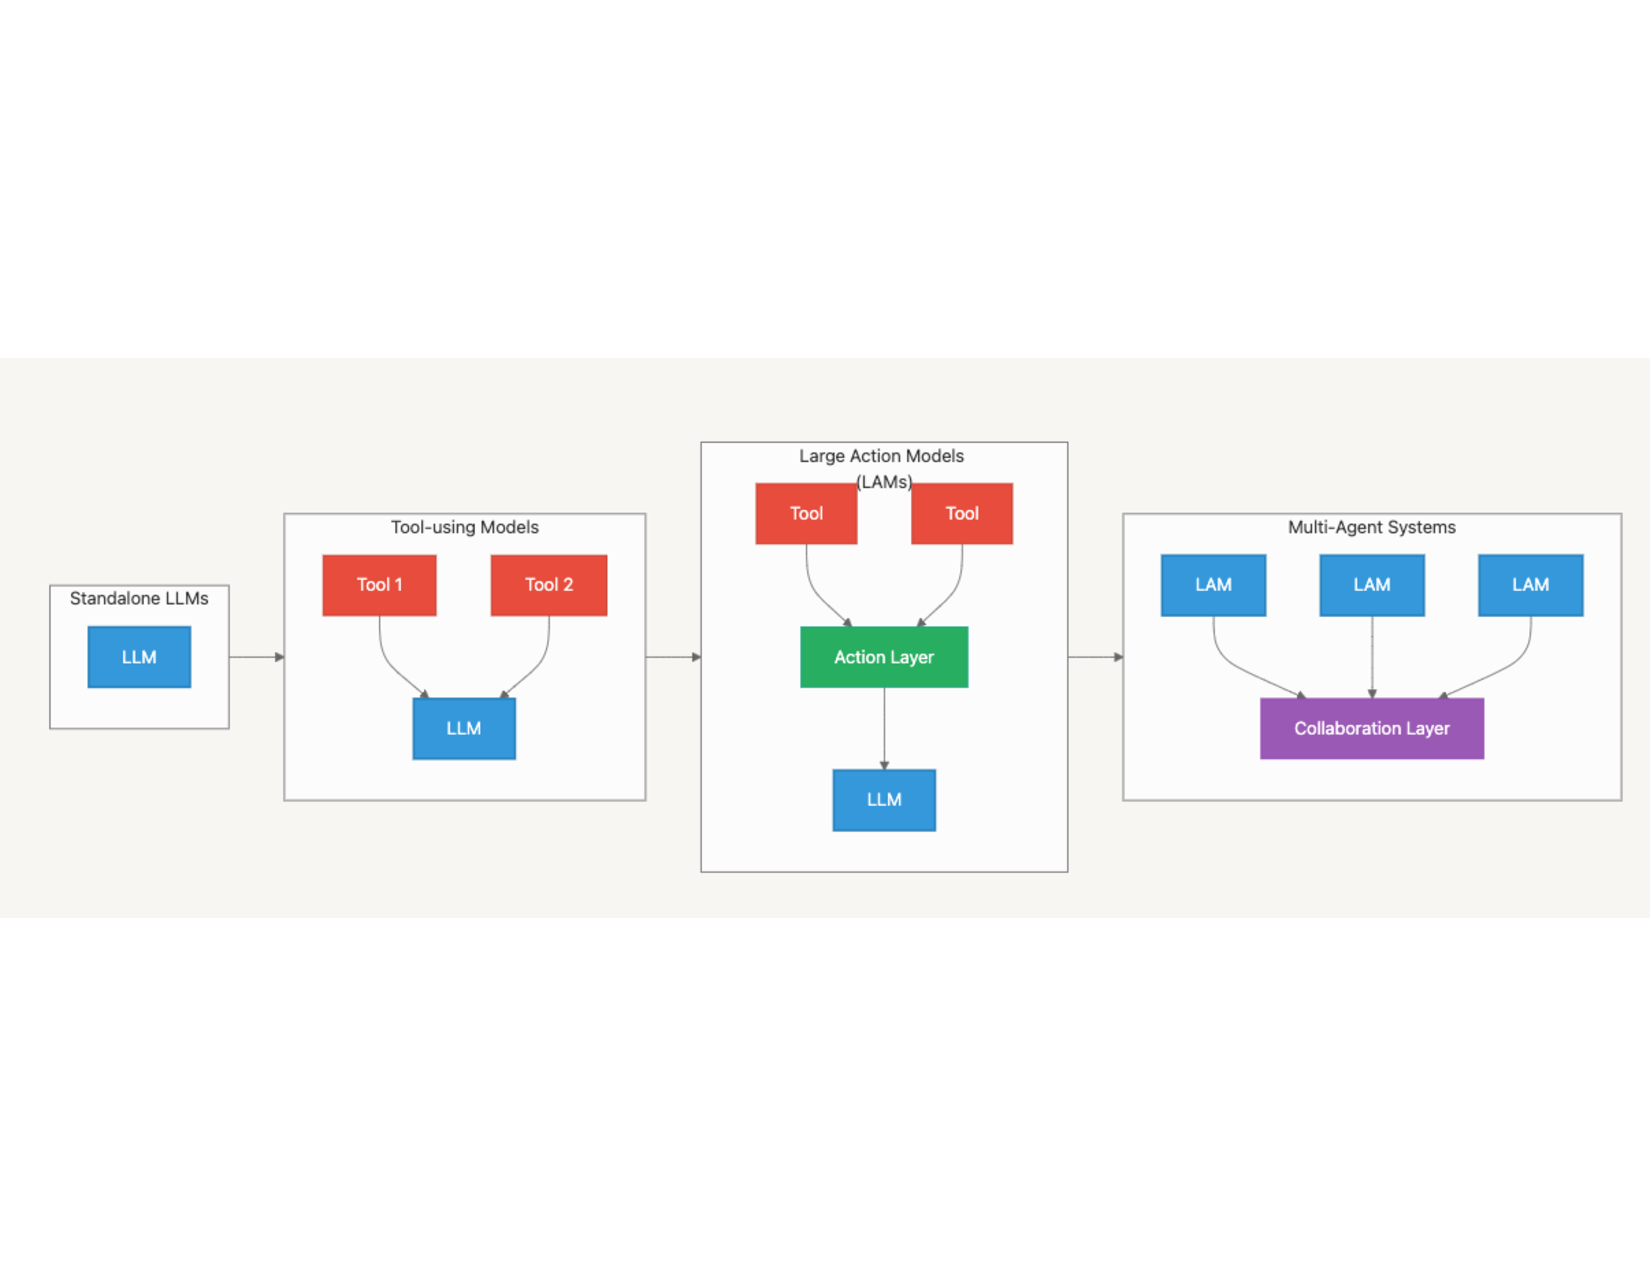
\includegraphics[width=0.5\textwidth, trim=0 150pt 0 150pt, clip]{lams_diagram.pdf}
    \caption{Evolution of AI systems from standalone LLMs to multi-agent systems.}
    \label{fig:lam-evolution}
\end{figure}

Let's take a brief pause and look at how our initial systems has evolved over time. First, we had LLM models that learned to use simple tools. Next, with more training, these models became better at making plans and developing strategies. Finally, when we combined these models with special helper programs (called agents), they got much better at doing real-world tasks. Based on our research, this combination of smart AI models working together with a layer of multi agent systems is likely to be the future of AI. When we give an AI model the right set of tools and helper programs, it can do a much better job of completing all kinds of tasks. 

This collaborative approach fundamentally transforms how AI operates by shifting from isolated models toward interconnected systems that can distribute complex problems. If the challenge with LAMs  was to design specific training to specialize our LLM, now the challenge for multi agent systems is to stablish roboust methods for a collaboration layer, which should enable them to communicate, coordinate, and collectively tackle complex, multi-step challenges. The following section will try to bring an overview of this important collaboration layer component.

According with \cite{tran2025multiagent}, the collaboration mechanisms in these systems can take various forms: Cooperation, competition and an hybrid approach named Coopetition. In cooperative scenarios, agents align their individual objectives with shared goals, often specializing in complementary roles to enhance efficiency. This approach has proven successful in applications ranging from question answering to collaborative programming, where different agents may handle research, planning, execution, and evaluation tasks. By contrast, competitive collaboration occurs when agents operate with potentially conflicting objectives, which can drive innovation and robustness through evolutionary pressure. Such competition-based approaches have shown benefits in debate frameworks and strategic gaming environments, where contradictory perspectives often yield more nuanced and comprehensive solutions. A hybrid approach—coopetition—enables agents to collaborate on certain tasks while competing on others, facilitating negotiation and compromise in complex, multi-objective problems.

Communication is another important part component of collaboration as it defines the information flow between agents. In centralized architectures, communication follows a star structure  where interactions flow through a central coordinator agent that manages task allocation and synthesizes results. On the other hand decentralized structures enable peer-to-peer interactions without centralized control, offering greater resilience against single points of failure, altough there is a downside, as more sophisticated coordination mechanisms are required. The communication system could also have a hierarchical arrangement by creating layered structures with defined authority levels, this balance control and flexibility across different tiers of agents with varying specializations.

In our research, we noticed significant enthusiasm for agentic systems across various tech communities. Through examining relevant papers, we identified that successful implementation and adoption of these systems depends heavily on addressing key challenges outlined in this paper. For example, to make these communication structures work effectively, a common protocol must be defined. This protocol should accommodate three essential factors that govern AI agent collaboration:

1. It should be rule-based: Having clear, predefined guidelines that specify how agents interact with each other
2. It should allow for role-based systems: Assigning different jobs to different agents based on their specific capabilities
3. Flexible systems: Enabling behavior adjustment based on changing situations and uncertainties

These systems ensure AI agents collaborate in an organized and effective manner. We expect to see more solutions addressing this key challenge in the coming year. It's worth noting Anthropic's Model Context Protocol (MCP) which, despite lacking academic publication, demonstrates promising adoption and usability in addressing the previously discussed challenges.

\subsection{Applications and Use Cases}
Recent advances in AI systems have led to practical applications across various domains. The evolution from LLMs to LAMs and beyond has created a rich ecosystem of specialized models with distinct capabilities:
Large Action Models (LAMs)
LAMs have emerged as powerful tools for structured decision-making environments. These models typically consist of a state encoder for processing structured input, a policy network for generating actions, and a value network to estimate expected rewards. Notable examples include:

xLAM – A Family of Large Action Models: The xLAM series, pioneered by Salesforce, exemplifies how LAMs can empower AI agent systems \cite{zhang2024xlam}. These models, spanning various sizes and architectures, have demonstrated excellence in executing real-world tasks, including tool use and interactive operations.
Game AI Systems: DeepMind's AlphaGo was the first AI to defeat a human champion at Go, utilizing deep neural networks with Monte Carlo Tree Search (MCTS) to evaluate board states and optimize long-term strategies \cite{silver2016mastering}.
Complex Game Environments: OpenAI Five leveraged self-play and Proximal Policy Optimization to master the multiplayer game Dota 2, demonstrating LAMs' ability to handle complex, dynamic environments with multiple agents \cite{openai2019dota}.
Autonomous Driving: Companies like Waymo employ convolutional neural networks to interpret sensor data (LIDAR, cameras) alongside reinforcement learning-based planning frameworks to produce driving behaviors \cite{bojarski2016end}. Similarly, Tesla's Full Self-Driving system utilizes transformer-based neural networks that process multiple input streams simultaneously to make real-time driving decisions \cite{lambert2023tesla}. 

\section{Future Directions} 


The evolution from isolated language models to integrated multi-agent systems represents a pivotal transformation in artificial intelligence capabilities. While impressive strides have been made, the journey ahead presents several critical challenges that must be addressed to unlock the full potential of these systems. As we envision the future landscape of AI agents, we see a progressive path where advances in several interconnected areas will collectively drive the field forward.

The foundation of effective multi-agent systems begins with sophisticated task planning and coordination mechanisms. Current approaches struggle to optimally distribute responsibilities across agents with specialized capabilities, particularly as system complexity increases. Future research must develop dynamic allocation algorithms that understand not only what each agent can do but when it should do it. The introduction of structured debate loops, where agents iteratively refine intermediate results through collaborative reasoning, shows particular promise. These approaches, potentially guided by game-theoretic frameworks like Stackelberg or Nash equilibria, could dramatically enhance collective problem-solving capabilities.

As these coordination mechanisms evolve, they must be supported by increasingly sophisticated memory and context management systems. Unlike single-agent frameworks, multi-agent systems must juggle multiple layers of context—from agent-specific knowledge to shared consensus information. This introduces unique challenges in maintaining contextual alignment across agents while preserving the integrity of private information. The development of hierarchical memory architectures with appropriate access controls, along with advanced episodic memory systems that learn from past collaborative interactions, will prove crucial for coherent system operation.

The bridges between these islands of specialized intelligence—communication frameworks—require equal attention. Current systems often suffer from inefficient information exchange that creates bottlenecks as agent populations grow. Standardized protocols that enable seamless integration of diverse agent types, coupled with sophisticated negotiation and consensus-building mechanisms, will be essential for scaling these systems beyond simple demonstrations to robust, production-ready applications.

As multi-agent systems grow in complexity and scope, concerns about reliability and resilience become increasingly pressing. Methods for preventing error propagation, ensuring graceful degradation when individual agents fail, and dynamically integrating new agents into operational systems will be necessary to maintain trust in these increasingly autonomous frameworks. This technical robustness must be paired with comprehensive evaluation methodologies—an area where current research falls notably short. The field urgently needs metrics and benchmarks specifically designed to assess collaborative performance and emergent system capabilities, not just individual agent effectiveness.

The application of these advances to specific domains presents both unique challenges and opportunities. The integration of multi-agent systems with blockchain technologies, as highlighted in recent research [7], offers promising directions for enhancing distributed system capabilities. Similarly, embedding these systems within enterprise software ecosystems or bridging digital reasoning with physical action through robotics presents domain-specific hurdles that will require specialized research attention.

Addressing these interconnected challenges demands collaborative efforts spanning artificial intelligence, distributed systems, human-computer interaction, and domain expertise. As researchers tackle these problems, we anticipate a gradual transition from today's experimental prototypes to tomorrow's production-ready systems—systems capable of reliably executing complex, collaborative tasks across diverse real-world environments. This transition will not only advance technological capabilities but potentially redefine how we conceptualize the boundaries between human and artificial intelligence in productive work.

\section{Conclusion}
The evolution from large language models to multi-agent systems represents a fundamental transformation in AI capabilities. This journey—from text generation to autonomous action execution—has progressed through distinct stages: tool-using LLMs that identified when to leverage external functionalities; specialized Large Action Models (LAMs) trained to execute complex task sequences; and collaborative multi-agent systems where specialized agents work together to solve problems beyond individual capabilities.
This progression has expanded AI's practical utility across domains, enabling sophisticated automation previously requiring human intervention. However, significant challenges remain in coordination mechanisms, communication protocols, error resilience, and evaluation methodologies. Future research must focus on developing robust frameworks for agent collaboration, standardized communication, and comprehensive performance metrics tailored for multi-agent interactions.
As these systems mature, we anticipate a shift from experimental prototypes to production-ready applications capable of executing complex, collaborative tasks in diverse real-world environments. This transition will not only advance technological capabilities but may fundamentally redefine human-AI collaboration in productive work across industries—from software development to creative content generation to strategic decision-making.

\bibliographystyle{IEEEtran}
\bibliography{references}
 
\end{document}